\documentclass{article}
% \documentclass[10pt]{article}
\usepackage[margin=1.7in]{geometry}
\usepackage{etoolbox}
\pagenumbering{arabic}
% \usepackage{amssymb}
\usepackage{amsmath}
\usepackage{amsthm}
% \usepackage{amsfonts}
\usepackage[pdfstartview=FitH,colorlinks,urlcolor=black,linkcolor=black,citecolor=black,pdfpagelabels,bookmarksdepth=2,bookmarksopen=true,bookmarksnumbered]{hyperref}
\usepackage{changepage}

% Easter egg: "The best way to keep a secret is to never have it." - Bruce Schneier

\usepackage[notcomma,notperiod,notquote,notcolon,notexcl,notquery,notscolon]{hanging}

\usepackage[capitalise,noabbrev]{cleveref}
%\usepackage[margin=1.5in]{geometry}
\usepackage[parfill]{parskip}
\usepackage[normalem]{ulem}
\usepackage{framed}
\usepackage{xcolor}
\usepackage{pagecolor,lipsum}
\usepackage{bold-extra}
\usepackage{caption}

\newcommand{\concat}{\mathbin{||}}
\newcommand{\inputs}{\mathsf{inputs}}

%fields and groups
\newcommand{\id}{\mathsf{id}}
\newcommand{\overflow}{\mathsf{overflow}}
\newcommand{\F}{\mathbb{F}}
\newcommand{\Fp}{\F_p}
\newcommand{\Fq}{\F_q}
\newcommand{\Ftwo}{\F_2}
\newcommand{\Q}{\mathbb{Q}}
\newcommand{\N}{\mathbb{N}}
\newcommand{\Z}{\mathbb{Z}}
\newcommand{\R}{\mathbb{R}}
\newcommand{\C}{\mathbb{C}}
\newcommand{\T}{\mathbb{T}}
\newcommand{\Qbar}{\overline{\Q}}
\newcommand{\G}{\mathbb{G}}
\newcommand{\Vs}{\mathbb{V}}
\newcommand{\Fbar}{\overline{\mathbb{F}}}
\newcommand{\Hash}{\mathsf{Hash}}
\newcommand{\Omtilde}{\widetilde{\Omega}}

\newcommand{\Enc}{\mathsf{Enc}}
\newcommand{\Dec}{\mathsf{Dec}}
\renewcommand{\DH}{\mathsf{DH}}
\newcommand{\gen}{\mathsf{Gen}}
\newcommand{\enc}{\Enc}
\newcommand{\dec}{\Dec}

\DeclareMathOperator*{\E}{\textrm{E}}

\DeclareMathOperator*{\Dima}{\textrm{Dima}}


%vectors, etc.
\newcommand{\av}{\mathbf{a}} \newcommand{\cv}{\mathbf{c}}
\newcommand{\dv}{\mathbf{d}} \newcommand{\ev}{\mathbf{e}}
\newcommand{\rv}{\mathbf{r}} \newcommand{\sv}{\mathbf{s}}
\newcommand{\tv}{\mathbf{t}} \newcommand{\uv}{\mathbf{u}}
%\newcommand{\vv}{\mathbf{v}} \newcommand{\wv}{\mathbf{w}}
\newcommand{\xv}{\mathbf{x}} \newcommand{\yv}{\mathbf{y}}
\newcommand{\zv}{\mathbf{z}} \newcommand{\zerov}{\mathbf{0}}
\renewcommand{\AA}{\mathbf{A}} \newcommand{\BB}{\mathbf{B}}
\newcommand{\CC}{\mathbf{C}} \newcommand{\FF}{\mathbf{F}}
\newcommand{\MM}{\mathbf{M}} \newcommand{\RR}{\mathbf{R}}
\renewcommand{\SS}{\mathbf{S}} \newcommand{\TT}{\mathbf{T}}
\newcommand{\UU}{\mathbf{U}} \newcommand{\XX}{\mathbf{X}}
\newcommand{\YY}{\mathbf{Y}} \newcommand{\KK}{\mathbf{K}}
\newcommand{\A}{\mathcal{A}} \newcommand{\B}{\mathcal{B}}
\newcommand{\dash}{\mbox{---}}
\renewcommand{\O}{\mathcal{O}}
\newcommand{\qq}{\mathfrak{q}}
\newcommand{\QQ}{\mathfrak{Q}}
\newcommand{\ZQ}{\Z_{q}}

\newcommand{\vu}{\mathbf{u}}

\newcommand{\todo}[1]{{\color{red}[\textbf{TODO}: #1]}}

\newcommand{\mr}[1]{\ensuremath{\mathrm{{#1}}}}
\newcommand{\la}{\ensuremath{\leftarrow}}
\newcommand{\ra}{\ensuremath{\rightarrow}}
\newcommand{\ala}{\ensuremath{\ \la\ }}
\newcommand{\ara}{\ensuremath{\ \ra\ }}
\newcommand{\rf}{\ensuremath{\overset{\$}{\la}}}

\newcommand{\calA}{\ensuremath{\mathcal{A}}}
\newcommand{\calB}{\ensuremath{\mathcal{B}}}
\newcommand{\calC}{\ensuremath{\mathcal{C}}}
\newcommand{\calD}{\ensuremath{\mathcal{D}}}
\newcommand{\calE}{\ensuremath{\mathcal{E}}}
\newcommand{\calF}{\ensuremath{\mathcal{F}}}
\newcommand{\calG}{\ensuremath{\mathcal{G}}}
\newcommand{\calH}{\ensuremath{\mathcal{H}}}
\newcommand{\calI}{\ensuremath{\mathcal{I}}}
\newcommand{\calJ}{\ensuremath{\mathcal{J}}}
\newcommand{\calK}{\ensuremath{\mathcal{K}}}
\newcommand{\calL}{\ensuremath{\mathcal{L}}}
\newcommand{\calM}{\ensuremath{\mathcal{M}}}
\newcommand{\calN}{\ensuremath{\mathcal{N}}}
\newcommand{\calO}{\ensuremath{\mathcal{O}}}
\newcommand{\calP}{\ensuremath{\mathcal{P}}}
\newcommand{\calQ}{\ensuremath{\mathcal{Q}}}
\newcommand{\calR}{\ensuremath{\mathcal{R}}}
\newcommand{\calS}{\ensuremath{\mathcal{S}}}
\newcommand{\calT}{\ensuremath{\mathcal{T}}}
\newcommand{\calU}{\ensuremath{\mathcal{U}}}
\newcommand{\calV}{\ensuremath{\mathcal{V}}}
\newcommand{\calW}{\ensuremath{\mathcal{W}}}
\newcommand{\calX}{\ensuremath{\mathcal{X}}}
\newcommand{\calY}{\ensuremath{\mathcal{Y}}}
\newcommand{\calZ}{\ensuremath{\mathcal{Z}}}

% -- bold math symbols, for some reason --
\newcommand{\boldalpha}{\ensuremath{\boldsymbol{\alpha}}}
\newcommand{\boldchi}{\ensuremath{\boldsymbol{\chi}}}
\newcommand{\boldtau}{\ensuremath{{\boldsymbol{\tau}}}}
\newcommand{\boldstar}{\ensuremath{\mathbf{*}}}
\newcommand{\bolda}{\ensuremath{\mathbf{a}}}
\newcommand{\boldb}{\ensuremath{\mathbf{b}}}
\newcommand{\boldc}{\ensuremath{\mathbf{c}}}
\newcommand{\boldd}{\ensuremath{\mathbf{d}}}
\newcommand{\bolde}{\ensuremath{\mathbf{e}}}
\newcommand{\boldf}{\ensuremath{\mathbf{f}}}
\newcommand{\boldg}{\ensuremath{\mathbf{g}}}
\newcommand{\boldh}{\ensuremath{\mathbf{h}}}
\newcommand{\boldi}{\ensuremath{\mathbf{i}}}
\newcommand{\boldj}{\ensuremath{\mathbf{j}}}
\newcommand{\boldk}{\ensuremath{\mathbf{k}}}
\newcommand{\boldl}{\ensuremath{\mathbf{l}}}
\newcommand{\boldm}{\ensuremath{\mathbf{m}}}
\newcommand{\boldn}{\ensuremath{\mathbf{n}}}
\newcommand{\boldo}{\ensuremath{\mathbf{o}}}
\newcommand{\boldp}{\ensuremath{\mathbf{p}}}
\newcommand{\boldq}{\ensuremath{\mathbf{q}}}
\newcommand{\boldr}{\ensuremath{\mathbf{r}}}
\newcommand{\bolds}{\ensuremath{\mathbf{s}}}
\newcommand{\boldt}{\ensuremath{\mathbf{t}}}
\newcommand{\boldu}{\ensuremath{\mathbf{u}}}
\newcommand{\boldv}{\ensuremath{\mathbf{v}}}
\newcommand{\boldw}{\ensuremath{\mathbf{w}}}
\newcommand{\boldx}{{\ensuremath{\mathbf{x}}}}
\newcommand{\boldy}{\ensuremath{\mathbf{y}}}
\newcommand{\boldz}{\ensuremath{\mathbf{z}}}
\newcommand{\boldzero}{\ensuremath{\boldsymbol{0}}}
\newcommand{\boldone}{\ensuremath{\boldsymbol{1}}}
\newcommand{\boldpi}{\ensuremath{\boldsymbol{\pi}}}
\newcommand{\boldPi}{\ensuremath{\boldsymbol{\Pi}}}

% -- bold italic math symbols, for some reason --
\newcommand{\boldia}{\ensuremath{\boldsymbol{a}}}
\newcommand{\boldib}{\ensuremath{\boldsymbol{b}}}
\newcommand{\boldic}{\ensuremath{\boldsymbol{c}}}
\newcommand{\boldid}{\ensuremath{\boldsymbol{d}}}
\newcommand{\boldie}{\ensuremath{\boldsymbol{e}}}
\newcommand{\boldif}{\ensuremath{\boldsymbol{f}}}
\newcommand{\boldig}{\ensuremath{\boldsymbol{g}}}
\newcommand{\boldih}{\ensuremath{\boldsymbol{h}}}
\newcommand{\boldii}{\ensuremath{\boldsymbol{i}}}
\newcommand{\boldij}{\ensuremath{\boldsymbol{j}}}
\newcommand{\boldik}{\ensuremath{\boldsymbol{k}}}
\newcommand{\boldil}{\ensuremath{\boldsymbol{l}}}
\newcommand{\boldim}{\ensuremath{\boldsymbol{m}}}
\newcommand{\boldin}{\ensuremath{\boldsymbol{n}}}
\newcommand{\boldio}{\ensuremath{\boldsymbol{o}}}
\newcommand{\boldip}{\ensuremath{\boldsymbol{p}}}
\newcommand{\boldiq}{\ensuremath{\boldsymbol{q}}}
\newcommand{\boldir}{\ensuremath{\boldsymbol{r}}}
\newcommand{\boldis}{\ensuremath{\boldsymbol{s}}}
\newcommand{\boldit}{\ensuremath{\boldsymbol{t}}}
\newcommand{\boldiu}{\ensuremath{\boldsymbol{u}}}
\newcommand{\boldiv}{\ensuremath{\boldsymbol{v}}}
\newcommand{\boldiw}{\ensuremath{\boldsymbol{w}}}
\newcommand{\boldix}{\ensuremath{\boldsymbol{x}}}
\newcommand{\boldiy}{\ensuremath{\boldsymbol{y}}}
\newcommand{\boldiz}{\ensuremath{\boldsymbol{z}}}

\newcommand{\transpose}[1]{\ensuremath{{#1}^{\intercal}}}

\newcommand{\boldA}{\ensuremath{\mathbf{A}}}
\newcommand{\boldB}{\ensuremath{\mathbf{B}}}
\newcommand{\boldC}{\ensuremath{\mathbf{C}}}
\newcommand{\boldD}{\ensuremath{\mathbf{D}}}
\newcommand{\boldE}{\ensuremath{\mathbf{E}}}
\newcommand{\boldF}{\ensuremath{\mathbf{F}}}
\newcommand{\boldG}{\ensuremath{\mathbf{G}}}
\newcommand{\boldH}{\ensuremath{\mathbf{H}}}
\newcommand{\boldI}{\ensuremath{\mathbf{I}}}
\newcommand{\boldJ}{\ensuremath{\mathbf{J}}}
\newcommand{\boldK}{\ensuremath{\mathbf{K}}}
\newcommand{\boldL}{\ensuremath{\mathbf{L}}}
\newcommand{\boldM}{\ensuremath{\mathbf{M}}}
\newcommand{\boldN}{\ensuremath{\mathbf{N}}}
\newcommand{\boldO}{\ensuremath{\mathbf{O}}}
\newcommand{\boldP}{\ensuremath{\mathbf{P}}}
\newcommand{\boldQ}{\ensuremath{\mathbf{Q}}}
\newcommand{\boldR}{\ensuremath{\mathbf{R}}}
\newcommand{\boldS}{\ensuremath{\mathbf{S}}}
\newcommand{\boldT}{\ensuremath{\mathbf{T}}}
\newcommand{\boldU}{\ensuremath{\mathbf{U}}}
\newcommand{\boldV}{\ensuremath{\mathbf{V}}}
\newcommand{\boldW}{\ensuremath{\mathbf{W}}}
\newcommand{\boldX}{\ensuremath{\mathbf{X}}}
\newcommand{\boldY}{\ensuremath{\mathbf{Y}}}
\newcommand{\boldZ}{\ensuremath{\mathbf{Z}}}

\newcommand{\defeq}{\overset{\text{\tiny def}}{=}}
\newcommand{\deq}{\defeq}
\newcommand{\zo}{\ensuremath{\{0,1\}}} % bits
\newcommand{\zon}{\ensuremath{\{0,1\}^n}} % bits

% Theorem definitions

\theoremstyle{plain}
\newtheorem{theorem}{Theorem}[section]
\newtheorem*{rtheorem}{Theorem}
\newtheorem{lemma}[theorem]{Lemma}
\newtheorem{prop}[theorem]{Proposition}
\newtheorem{corollary}[theorem]{Corollary}
\theoremstyle{remark}
\newtheorem*{remark}{Remark}
\theoremstyle{definition}
\newtheorem*{claims}{Claim}
\newtheorem*{theorems}{Theorem}
\newtheorem{defn}[theorem]{Definition}
\newtheorem{definition}[theorem]{Definition}
\newtheorem{fact}[theorem]{Fact}
\newtheorem{conjecture}[theorem]{Conjecture}
\newtheorem{const}[theorem]{Construction}
\newtheorem{attackgame}[theorem]{Attack Game}


\newtheoremstyle{goal}% name of the style to be used
  {\topsep}% measure of space to leave above the theorem. E.g.: 3pt
  {\topsep}% measure of space to leave below the theorem. E.g.: 3pt
  {\normalfont}% name of font to use in the body of the theorem
  {0pt}% measure of space to indent
  {\bfseries}% name of head font
  {: } %punctuation between head and body
  { }% space after theorem head; " " = normal interword space
  {\thmname{#1}\thmnumber{ #2}\thmnote{ (#3)}}
\theoremstyle{goal}
\newtheorem{sgoal}{Security Goal}
\newtheorem{fgoal}{Functionality Goal}

%% custom macros

\newcommand{\Perms}{\operatorname{perms}}
\newcommand{\esm}[1]{\ensuremath{#1}}
\newcommand{\ms}[1]{\esm{\mathsf{#1}}}

\newcommand{\compind}{\appc}
\newcommand{\prg}{\ms{PRG}}
\newcommand{\prf}{\ms{PRF}}
\newcommand{\prp}{\ms{PRP}}

\newcommand{\poly}{\operatorname{poly}}
\newcommand{\polylog}{\operatorname{polylog}}
\newcommand{\negl}{\operatorname{negl}}

\newcommand{\hyb}{\ms{Hyb}}
\newcommand{\Funs}{\ms{Funs}}
\newcommand{\getsr}{\rgets}
\newcommand{\rgets}{\mathrel{\mathpalette\rgetscmd\relax}}
\newcommand{\rgetscmd}{\ooalign{$\leftarrow$\cr
    \hidewidth\raisebox{1.2\height}{\scalebox{0.5}{\ \rm R}}\hidewidth\cr}}

%\getsr with proper vertical space.    
% this makes it typeset better in subscripts
\def\getsrx{\mathrel{%
    \mathchoice{\GETSRX}{\GETSRX}{\scriptsize\GETSRX}{\tiny\GETSRX}%
}}
\def\GETSRX{{%
\setbox0\hbox{$\gets$}%
\rlap{\hbox to \wd0{\hss$\raisebox{1.2\height}{\scalebox{0.5}{\ R}}$\hss}}\box0
}}

\newcommand{\Unif}{\ms{Unif}}

\newcommand{\iseq}{\stackrel{?}{=}}

\newcommand{\appc}{\stackrel{c}{\approx}}
\newcommand{\apps}{\stackrel{s}{\approx}}
\newcommand{\abs}[1]{\left| #1 \right|}

\newcommand{\classP}{\ms{P}}
\newcommand{\classBPP}{\ms{BPP}}
\newcommand{\classNP}{\ms{NP}}
\newcommand{\Ppoly}{\ms{P}/\ms{poly}}
\newcommand{\NCone}{\ms{NC^1}}

\newcommand{\round}[1]{\left\lfloor #1 \right\rceil}
\newcommand{\floor}[1]{\left\lfloor #1 \right\rfloor}
\newcommand{\ceil}[1]{\left\lceil #1 \right\rceil}
\newcommand{\iprod}[1]{\left\langle #1 \right\rangle}
\newcommand{\norm}[1]{\left\| #1 \right\|}
\newcommand{\set}[1]{\left\{ #1 \right\}}

\newcommand{\Zp}{\Z_p}
\newcommand{\Zq}{\Z_q}

\newcommand{\subind}[2]{{#1}^{(#2)}}

\newcommand{\eqq}{\stackrel{?}{=}}

\newcommand{\Otilde}{\widetilde{O}}
\newcommand{\Otildel}{\widetilde{O}_\lambda}
\newcommand{\Omtildel}{\widetilde{\Omega}_\lambda}

\newcommand{\hc}{\ms{hc}}

\newcommand{\xstar}{x^*}
\newcommand{\ystar}{y^*}

\newcommand{\DDHAdv}{\ms{DDHAdv}}
\newcommand{\PRFAdv}{\ms{PRFAdv}}
\newcommand{\PRGAdv}{\ms{PRGAdv}}

\newcommand{\ct}{\ms{ct}}

\newcommand{\View}{\ms{View}}
\newcommand{\view}{\View}
%\newcommand{\view}{\ms{View}_{\calV^*}}
\newcommand{\Sim}{\ms{Sim}}


\newcommand{\bv}{\mathbf{b}}
\newcommand{\Bm}{\mathbf{B}}
\newcommand{\Rm}{\mathbf{R}}
\newcommand{\Gm}{\mathbf{G}}

\newcommand{\pro}[1]{\langle #1 \rangle}
\newcommand{\Comm}{\ms{Commit}}
\newcommand{\cSAT}{\ms{circuit}\text{-}\ms{SAT}}

\newcommand{\op}{\ms{op}}
\newcommand{\ck}{\ms{ck}}
\newcommand{\st}{\ms{st}}

\newcommand{\sk}{{\ms{sk}}}
\newcommand{\pk}{\ms{pk}}

\newcommand{\ol}{1^{\lambda}}
\newcommand*{\Zpos}{\Zgz}


%%%%
% Custom stuff
\newcommand{\Route}{\mathsf{Route}}
\newcommand*{\algcomment}[1]{\texttt{\null\hfill\small {\color{gray} // #1}}}
\newcommand{\keyspace}{\calK}
\newcommand{\msgspace}{\calM}
\newcommand{\ctspace}{\calC}
\newcommand{\prfkey}{k}
\newcommand{\xor}{\oplus}
% crypto and math commands 
\newcommand{\diam}{\operatorname{diam}}

\newcommand{\setup}{\mathsf{Setup}}
\newcommand{\rte}{\mathsf{Route}}
\newcommand{\dist}{\mathsf{Distribute}}

\newcommand{\pir}{\mathsf{PIR}}
\newcommand{\query}{\mathsf{PIR.Query}}
\newcommand{\answer}{\mathsf{PIR.Answer}}
\newcommand{\decode}{\mathsf{PIR.Decode}}
\newcommand{\queries}{\mathsf{queries}}
\newcommand{\slot}{\mathsf{slot}}
\newcommand{\slots}{\mathsf{slots}}
\newcommand{\keys}{\mathsf{keys}}
\newcommand{\pred}{\mathsf{pred}}
\newcommand{\data}{\mathsf{data}}
\newcommand{\db}{\mathsf{db}}
\newcommand{\predIndex}{\mathsf{predIndex}}
\newcommand{\indexOf}{\mathsf{indexOf}}
\newcommand{\predSlot}{\mathsf{predSlot}}
%\renewcommand{\Cap}{\mathsf{cap}}
\newcommand{\rows}{\mathsf{rows}}
\newcommand{\SetupHelp}{\mathsf{SetupHelp}}
\newcommand{\Dreal}{\calD_\text{real}}
\newcommand{\Dideal}{\calD_\text{ideal}}
\newcommand{\Cpp}{C\nolinebreak\hspace{-.05em}\raisebox{.1ex}{+}\nolinebreak\hspace{-.10em}\raisebox{.1ex}{+}\xspace}

\newcommand{\pdtuple}{(\setup,\allowbreak \dist, \allowbreak \dec)}

\newcommand{\kx}{\mathsf{kx}}
\newcommand{\ki}{\mathsf{ki}}
\renewcommand{\id}{\mathsf{id}}
\newcommand{\inv}{\mathsf{inv}}

% 🎉 EASTER EGGS: Cryptographic Fun Commands 🎉
% (Because even serious cryptographers need some humor!)

% Fun crypto-themed commands
\newcommand{\alice}{\textsc{Alice}} % Always capitalize our favorite cryptographer
\newcommand{\bob}{\textsc{Bob}}     % Bob deserves respect too
\newcommand{\eve}{\textsc{Eve}}     % The eternal eavesdropper
\newcommand{\mallory}{\textsc{Mallory}} % The malicious adversary

% Humorous security levels
\newcommand{\topsecret}[1]{\colorbox{black}{\textcolor{black}{#1}}} % Redacted text
\newcommand{\classified}[1]{\textbf{\textcolor{red}{[CLASSIFIED: #1]}}}
\newcommand{\burnaftereading}[1]{\textit{\textcolor{gray}{#1 \tiny{(burn after reading)}}}}

% Fun mathematical operators
\newcommand{\veryequal}{\stackrel{\text{very}}{=}} % For when = isn't emphatic enough
\newcommand{\secretlyequal}{\stackrel{\text{🤫}}{=}} % Shh, it's a secret equality
\newcommand{\probablyequal}{\stackrel{\text{probably}}{=}} % Cryptographic probability humor

% Anysphere-specific fun
\newcommand{\anysphere}{\textsc{Anysphere}} % Consistent branding
\newcommand{\metadata}{\textit{metadata}} % Emphasis on the star of the show
\newcommand{\pirmagic}{\textsc{PIR}$_{\text{✨}}$} % PIR with sparkles because it's magical
\newcommand{\homomorphicwizardry}{\textsc{Homomorphic Wizardry}} % Because HE is basically magic

% Security theater commands
\newcommand{\securitytheater}[1]{\textcolor{purple}{\textit{[Security Theater: #1]}}}
\newcommand{\actuallySecure}[1]{\textcolor{green}{\textbf{✓ Actually Secure: #1}}}

% Easter egg for the authors
\newcommand{\teamanysphere}{\textit{The Anysphere Cryptography Wizards}}

% Fun footnote commands
\newcommand{\cryptojoke}[1]{\footnote{\textit{Crypto joke: #1}}}
\newcommand{\nerdsnipe}[1]{\footnote{\textit{Nerd snipe: #1 (You're welcome for the distraction!)}}}

% The ultimate easter egg - a command that does nothing but exists
\newcommand{\illuminati}{\phantom{👁}} % The all-seeing eye... but invisible

% Quantum-safe humor (because why not?)
\newcommand{\quantumsafe}[1]{\textcolor{blue}{#1\textsuperscript{quantum-safe*}}}
\newcommand{\quantumvulnerable}[1]{\textcolor{orange}{#1\textsuperscript{⚠️ quantum-vulnerable}}}

% A command for when the math gets too intense
\newcommand{\mathintensifies}{\textit{[math intensifies]}}

% The classic "it's complicated" for cryptographic relationships
\newcommand{\itscomplicated}{\textit{(it's complicated)}}

% For those moments when you need to acknowledge the elephant in the room
\newcommand{\elephantinroom}[1]{\textcolor{gray}{\textit{[Elephant in room: #1]}}}

% A tribute to the unsung heroes of cryptography
\newcommand{\unsung}[1]{\textit{#1 (unsung hero of cryptography)}}

% Because sometimes you need to emphasize just how much you don't trust something
\newcommand{\donottrust}[1]{\textbf{\textcolor{red}{DO NOT TRUST: #1}}}
\newcommand{\trustwithyourlife}[1]{\textbf{\textcolor{green}{TRUST WITH YOUR LIFE: #1}}}

% The final easter egg - a command that celebrates making it to the end
\newcommand{\madeittotheend}{\textit{🎉 Congratulations! You found the end of the easter eggs! 🎉}}


\usepackage[lambda,adversary,advantage,asymptotics,sets,landau,probability,
    operators]{cryptocode}
\usepackage[style=alphabetic,backend=bibtex]{biblatex}
\addbibresource{bib.bib}
\usepackage[toc]{appendix}
\usepackage{ulem}

\usepackage{tikzsymbols}
\usetikzlibrary{decorations.pathreplacing}
\usetikzlibrary{calc}
\usetikzlibrary{hobby}
\usetikzlibrary{decorations.markings, decorations.pathmorphing}
\usetikzlibrary{shapes}
\usetikzlibrary{positioning,fit}

\createpseudocodeblock{pcb}{center, boxed}{}{}{}
\createprocedureblock{pcbexp}{center, boxed}{}{$\mathrm{Experiment}$\ }{}

\newcommand{\hcg}[1]{{\color{blue}[\textbf{HCG}: #1]}}
\newcommand{\oldhcg}[1]{{\color{gray}[\textbf{HCG}: #1]}}
\newcommand{\arvid}[1]{{\color{violet}[\textbf{AL}: #1]}}

\newcommand{\authtoken}{\pckeystyle{tk}}


\setcounter{tocdepth}{3}

%\renewcommand{\contentsnamefont}{\Large\raggedright\bfseries\MakeTextUppercase}

% Erik's \xxx macro
% Complex \xxx for making notes of things to do.  Use \xxx{...} for general
% notes, and \xxx[who]{...} if you want to blame someone in particular.
% Puts text in brackets and in bold font, and normally adds a marginpar
% with the text ``xxx'' so that it is easy to find.  On the other hand, if
% the comment is in a minipage, figure, or caption, the xxx goes in the text,
% because marginpars are not possible in these situations.
{\makeatletter
 \gdef\xxxmark{%
   \expandafter\ifx\csname @mpargs\endcsname\relax % in minipage?
     \expandafter\ifx\csname @captype\endcsname\relax % in figure/caption?
       \marginpar{xxx}% not in a caption or minipage, can use marginpar
     \else
       xxx % notice trailing space
     \fi
   \else
     xxx % notice trailing space
   \fi}
 \gdef\xxx{\@ifnextchar[\xxx@lab\xxx@nolab}
 \long\gdef\xxx@lab[#1]#2{\textbf{[\xxxmark #2 ---{\sc #1}]}}
 \long\gdef\xxx@nolab#1{\textbf{[\xxxmark #1]}}
 % This turns them off:
%  \long\gdef\xxx@lab[#1]#2{}\long\gdef\xxx@nolab#1{}%
}

% Counters
\newcounter{protocol-number}
\newcommand{\protocolNumber}{\refstepcounter{protocol-number}\arabic{protocol-number}}
\newcommand{\stzh}[1]{{\color{blue}[stzh: #1]}}

% 🥚 ULTIMATE EASTER EGG 🥚
% If you're reading this, you've found the secret message!
% 
% Dear future cryptographers and privacy advocates,
% 
% You've stumbled upon a whitepaper that represents a significant step forward
% in the quest for true digital privacy. Anysphere isn't just another messaging
% app - it's a glimpse into a future where your conversations are truly private,
% where metadata doesn't betray your secrets, and where "no needless trust"
% isn't just a slogan but a fundamental principle.
%
% The easter eggs scattered throughout this codebase are our way of saying:
% even the most serious cryptographic work deserves a smile. After all,
% if we can't have fun while building the future of privacy, what's the point?
%
% Remember: Alice and Bob have been trying to talk privately since 1976.
% Let's finally give them (and everyone else) the tools they deserve.
%
% Stay paranoid (in the best way),
% The Anysphere Team
%
% P.S. - If you found all the easter eggs, you deserve a coffee. ☕
% P.P.S. - Yes, we know there are probably bugs. It's crypto software. 🐛
% P.P.P.S. - The rubber duck debugging method works surprisingly well for PIR queries. 🦆

\title{\vspace{-2cm} \textbf{\Large Anysphere: Private Communication in Practice} \\ \vspace{0.3cm} {\large \normalfont Security Whitepaper} \vspace{-0.1cm}}
\def\dateinfo{July 6, 2022\\ \vspace{0.2cm} \textit{Last updated:} \today}
\date{\normalsize \dateinfo}
\author{\normalsize Arvid Lunnemark \hspace{0.7cm} Shengtong Zhang \hspace{0.7cm} Sualeh Asif \vspace{0.1cm} \\ \normalsize \nolinkurl{{arvid, stzh1555, sualeh}@anysphere.co}}

%\setshortauthors{Arvid Lunnemark, Shengtong Zhang, Sualeh Asif}
%\setshorttitle{Anysphere: Private Communication in Practice}

\makeatletter
\patchcmd{\@maketitle}{\begin{center}}{\begin{adjustwidth}{-0.5in}{-0.5in}\begin{center}}{}{}
\patchcmd{\@maketitle}{\end{center}}{\end{center}\end{adjustwidth}}{}{}
\makeatother

\begin{document}

\maketitle


\begin{abstract}
	\noindent We describe Anysphere, a metadata-private communication system deployed in the real world. By using private information retrieval based on homomorphic encryption, our protocol guarantees security even if all of our servers are compromised and any number of the users and network observers are malicious. In this whitepaper, we precisely define our threat model, and show how we achieve security against it both in theory and in practice.
\end{abstract}



%\tableofcontents

\section{Introduction}
\label{sec:introduction}

% When the internet was first established, everything sent over it was public. 
% If A sent a message to B, anyone on their path\stzh{route?} through the internet could see that such a message was sent, as well as read the actual message. As of today, many messaging services are end-to-end encrypted, meaning that no one can read the contents of messages. However, for sufficiently powerful adversaries — hackers, ISPs, government agencies — it is still possible to find out who is talking to whom, as well as when and how often messages are sent. Our goal is to hide this metadata: we want to create a system where A and B can send messages to each other over an untrusted network, without anyone knowing that they talk to each other. Such a private communication system would be critically important to protect and expand freedom in the world \cite{arvid}.

% From the start, Anysphere has assumed a single important security principle: \textit{no needless trust}. This simple principle guide Anysphere's development and is the key motivator behind our architecture, our threat model, and our choice of private information retrieval as our core protocol. 

% Quite simply, we believe that communication must place no needless trust in systems across the internet since many conversations are so meaningful\todo{impactful?} that unwarranted trust can lead to harm. In particular, we currently only trust the local device and your friends. That is it.

% Our principles are fundamentally different from Signal, Email, and other platforms and protocols that assume trust in the servers, in the plumbing of the internet, and in networks being so large that no entity can monitor them. We also solve many of the practical problems that plague research prototypes. We are working hard to make Anysphere more secure, and we are working hard to make it extremely security realistic for everyone.


% PLAN:

% paragraph 1: motivation

% what to convey?

% why should i care about metadata privacy?
    % can reveal a lot of information (quantify this? make it practical)
% what is metadata privacy?
    % ok this needs to go in first sentence
% start from the point of view of end-to-end encryption
    % this is important

% vibe:
% no alarmism please
% bitcoin whitepaper is... SO GOOD

% paragraph 2: what is needed is... no needless trust.

% what are you doing? (no needless trust)
% is what you are doing a paradigm shift? (yes)
% is this unique? (yes)




Electronic communication is a cornerstone of all interactions in the modern world, transforming individuals, organizations, and countries. Email, instant messaging, and video calls form the fundament of this electronic communication layer. Unfortunately, all these forms of electronic communication are not as secure or private as being in-person. Advances such as end-to-end encryption are significant for protecting \textit{what} is being said. Yet, information about who is talking to whom, how often, and when — \textit{the metadata} — is still being leaked at scale. Hackers, social media companies, and malicious nation-states have open access to the metadata, even for the most secure communication platforms on the market.

What is needed is a new approach: every part of every conversation must be protected, including metadata. The best, and possibly the only, way to protect metadata is not to give anyone access to it in the first place. Therefore, we operate on the principle of \textit{no needless trust}. Even if we could publish the passwords to our servers online, everyone's communication history and pattern would still be secure. This whitepaper accompanies our source code at {\tt \href{https://github.com/anysphere/client}{github.com/anysphere/client}}, and proves the security of Anysphere.
\section{Security Context}
\label{sec:securitycontext}

\todo{Explain why Signal is not enough. Good table.}

Signal is great. It is end-to-end encrypted, open source, and run by a trustworthy group. Unfortunately, if their servers are hacked, one of their employees bribed, or you are simply attacked by a network-level powerful actor, there is nothing Signal can guarantee.

\subsection{Goals}

\subsection{Threat Model}
\label{subsec:threatmodel}


We plan to achieve our goals in the presence of strong adversaries, whose capabilities we define in this section. Our belief in no needless trust means that our threat model is as extensive as possible.

%\begin{table*}[t]
%\centering
%another version below
%\begin{tabular}{||c c c c c c||} 
% \hline
%  Attacker compromises $\cdots$ & Anysphere & Signal & Skiff & Wickr & Onion  \\
% \hline
% Attacker listens on the internet & \checkmark & \checkmark & \checkmark & \checkmark \\ 
% \hline
% Attacker compromises & \checkmark & & & \checkmark & \checkmark \\
% \hline
% Skiff & \checkmark &  &  & & \checkmark\\
% \hline
% Wickr & \checkmark & & & \checkmark & \checkmark\\
% \hline
% Onion & \checkmark & *\footnote{\label{onion}Only guaranteed for non-global adversary} & &\checkmark&\checkmark\\
% \hline
%\end{tabular}
%\caption{Comparing when}
%\end{table*}

% \xxx{add an illustration of a walled garden, with the walls containing only your computer and your friends' computers} 

%Touch on: server, friends, client-side computer, etc.

\textbf{1. The attacker may compromise all servers.} To achieve privacy, we do not put any trust in the server. Our threat model assumes a global adversary who has full control over all servers, and can observe and manipulate all network traffic. This is similar to other anonymous communication schemes based on private information retrieval (for example \cite{ahmad2021addra}, \textsection 2.2), but stronger than most other anonymous communication schemes (e.g. Tor \cite{dingledine2004tor} and Nym \cite{piotrowska2017loopix}, which require partial trust in the servers).

\textbf{2. The attacker may control the entire internet.} See above.

\textbf{3. The attacker may compromise strangers.} We assume that the attacker has control over all clients that are not a contact of a given user, and can send maliciously crafted messages to and from these clients.

\textbf{4. The attacker cannot compromise contacts.} We assume that a user's contacts are trusted, and that the attacker does not have access to their computers. In \cite{angel2018s}, Angel, Lazar and Tzialla describe an attack on a general metadata-private communication system, which shows how to leak metadata in the presence of a compromised contact. The amount of metadata leaked to contacts is small, and we plan to look into measures for handling compromised contacts in the future (see \cref{sec:future}).
% that perfectly hiding metadata while not trusting the user's contacts is computationally prohibitive. <- edited out because we shouldnt have to justify not using this in the threat model.

\textbf{5. The attacker cannot access the user's computer.} We assume that a user's local computer is trusted and is running a correct implementation of our system. In \cref{sec:practical-security} we explain how we can relax this assumption slightly.

\textbf{6. The attacker cannot break standard cryptography.}: Our threat model assumes the security of the standard cryptography primitives we use. This includes Libsodium's AEAD implementation (XSalsa20), and Microsoft SEAL's homomorphic encryption implementation (BFV).

\subsection{Non-goals}
\textbf{1. Not a cryptocurrency.} Anysphere uses advanced cryptography, but not blockchains or cryptocurrencies.

\textbf{2. Not a plugin to an existing ecosystem.} Anysphere is not compatible with existing messaging systems like Signal or Email. This is intentional: interfacing with legacy systems would mean accepting their (much lower) standards of security and privacy.

\textbf{3. Not steganographic.} Anysphere does not make an attempt to hide who is using our service.


\section{Core Protocol}
\label{sec:coreprotocol}

Consider two fictional users, Alice and Bob. Alice and Bob want to message each other over an untrusted network without leaking any data or metadata to anyone. They use authenticated end-to-end encryption to hide the message content and ensure integrity. They employ two key ideas to hide metadata: sending data at a constant rate and retrieving homomorphically compressed data.

When signing up, each user gets their own \textit{outbox} on the server, which is a dedicated storage space for their messages. Once every minute, Alice sends exactly $1$ KB of data to her outbox. If she has a message to send, she sends the padded encryption of that message. Otherwise, she sends a random sequence of bytes. This simple idea ensures that neither the server nor network observers know when Alice sends a real message.

Our next problem is how to route the message to Bob. In a traditional messaging system, Bob downloads data from Alice's outbox and decrypts it. However, this leaks metadata: the server learns that Bob read from the Alice's outbox.

One solution is for Bob to, once every minute, download \textit{all} outboxes from the server. He can then check the value of Alice's outbox locally. This way, it is impossible for the server to link Alice to Bob.

This simplified scheme is almost how Anysphere works. Unfortunately, Bob cannot download all outboxes every minute — that would be too much data! Instead, he uses \textit{private information retrieval}, a well-studied cryptographic primitive, to compress his download size. \Cref{fig:highlevelpir} illustrates the core protocol. The following subsections will describe the system in detail.

% make this take up both columns at the top of the page
\begin{figure}
    \centering
    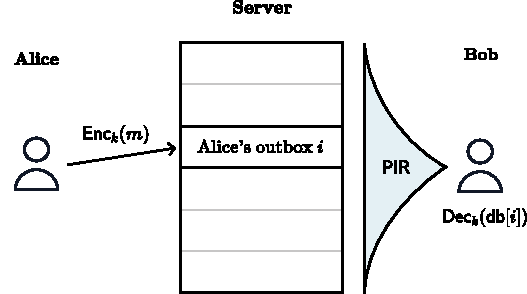
\includegraphics[width=0.7\textwidth]{pirfigure.pdf}
\caption{Alice sends the encryption of a message $m$ to her outbox once every minute. Bob retrieves Alice's outbox using private information retrieval (PIR), which appears to everyone else but Bob as if he had downloaded any outbox. Alice and Bob can use standard symmetric encryption to communicate, and the server will not learn anything at all.}
\label{fig:highlevelpir}
\end{figure}

\subsection{Private information retrieval}

We view the outboxes as an array, called $\db$. Bob wants to download Alice's outbox $\db[i]$ without revealing $i$ to anyone. This problem was first introduced as \textit{private information retrieval} (PIR) in 1995 \cite{chor1995private}, extended in 1997 to our threat model under the name cPIR \cite{kushilevitz1997replication}, and has been extensively studied since then \cite{melchor2016xpir,angel2018pir, ahmad2021addra}.

All known cPIR schemes use homomorphic encryption \cite{gentry2010computing}. To compute the query $q$, Bob encrypts $i$ with a homomorphic encryption scheme using a secret key $s$. That is, $q = \mathsf{HEnc}_s(i)$. The server can then homomorphically evaluate the function $f(i) = \db[i]$, producing the answer $a = \mathsf{HEnc}_s(\db[i])$. Bob can finally decrypt to find $\db[i]$. In practice, $f(i)$ is often defined in terms of a dot product with a unit vector representing $i$, because BFV, the homomorphic scheme being used, \cite{fan2012somewhat}, is particularly good at dot products.

Our implementation currently uses FastPIR, one of the fastest cPIR schemes \cite{ahmad2021addra}. All cPIR schemes have the same security properties, and we are actively researching faster schemes (see \cref{sec:future}).

\subsection{Security}

The simplest version of our core protocol is shown in \cref{fig:simple}. In this section, we show (1) that Alice and Bob enjoy metadata privacy without having to trust anyone else, (2) that our system guarantees message integrity, and (3) that our protocol is resistant to denial of service attacks from users.

We define security in the simulation sense \cite{lindell2017simulate}. To do so, we first need to define what an attacker learns, which includes both the data sent from all users to the server along with timestamps, as well as the local keys on attacker-controlled devices. Let $(S, i, \mathsf{tk}, c, t)$ represent the data sent to the server in the sending phase at time $t$, let $(R, q, t)$ represent the data sent to the server in the retrieving phase at time $t$, and let $(A, a, t)$ represent the data sent from the server in response to the retrieval request at time $t$. Our protocol does not operate in rounds, so $t$ can be any real number.

We say that a private communication scheme consists of the four algorithms $(\pcalgostyle{Register}, \mathsf{Send}, \mathsf{Receive}, \mathsf{Route})$, where $\pcalgostyle{Register}$ registers the user and generates a secret key

\begin{definition}[Metadata privacy]
    We say that a private communication scheme $(\pcalgostyle{Register}, \mathsf{Send}, \mathsf{Receive}, \mathsf{Route})$ is \textit{metadata-private} if for all $n = n_\lambda = \poly(\lambda)$, all $\mathcal{K} = \mathcal{K}_\lambda \subseteq [n]$, all $T = T_\lambda = \poly(\lambda)$, all user functions $m_u$, $t_u$ and $j_u$, all efficient attackers $\mathcal{S}$, and all efficient distinguishers $\mathcal{A}$, there exists an efficient algorithm $\mathsf{Sim}$, such that the following two probability ensembles, parametrized by $\lambda \in \N$, are computationally indistinguishable:
    \begin{align*}
        \Dreal &= \left\{ 
        \begin{aligned}
          (\{h_u^T\}_{u \in [n]}, &\{ \sk_u \}_{u \in \calK}, \{ t_u \}_{u \in [n]}) \colon \\
          \sk_u &\gets \pcalgostyle{Register}(1^\lambda, u) \;\; \forall u \in [n]\\
          h_u^0 &\gets \emptyset \;\; \forall u \in [n] \\
          s_u^{i+1} &\gets \mathsf{Send}(m_u(h_u^i), t_u(i), \sk_u) \;\; \forall u \notin \mathcal{K} \\
          q_u^{i+1} &\gets \mathsf{Retrieve}(j_u(h_u^i), t_u(i), \sk_u) \;\; \forall u \notin \mathcal{K} \\
          h_u^{i+1} &\gets h_u^i \cup s_u^{i+1} \cup q_u^{i+1}  \cup \mathcal{S}\left(H_t, q_u^{i+1}\right) \;\; \forall u \notin \mathcal{K} \\
          h_u^{i+1} &\gets h_u^i \cup \mathcal{S}(H_t) \;\; \forall u \in \mathcal{K}
        \end{aligned}\right\}_{\lambda \in \N}\\
        \Dideal &= \left\{
        \begin{aligned}
          \Sim\big(1^\lambda, \{h_u^T\}_{u \in \calK}, &\{ \sk_u \}_{u \in \calK}, \{ t_u \}_{u \in [n]}\big) \colon \\
          &(\{h_u^T\}_{u \in [n]}, \{ \sk_u \}_{u \in \calK}, \{ t_u \}_{u \in [n]}) \in \Dreal
        \end{aligned}
          \right\}_{\lambda \in \N},
      \end{align*}
      where \begin{equation*}
          H_t = \left\{(\cdot,\ldots,\cdot,t) \in \bigcup_{u, i} h_u^i : t < t_u(i)\right\}
      \end{equation*}
      is the global history up until time $t$.
\end{definition}

\textbf{Going offline.} Users will not always be connected to the internet. At night, most people put their computers to sleep. This means that users will not be sending and receiving exactly once every minute. \xxx{how much information does this leak?} \xxx[stzh]{To ensure security, we urge users to keep a regular transmission schedule by putting their computers asleep at a regular time each day.}

\textbf{Authentication token.} 
On registration, the server creates a unique authentication token for the new user. This allows the server to restrict access to that user's outbox, preventing denial of service attacks from other users. It should still be noted that, in accordance with our threat model, we do not prevent against denial of service attacks by ISPs or the server itself — fundamentally, a powerful actor can always shut down your internet access. In \cref{sec:future} we discuss plans for distributing the server such that, say, only 1 out of 3 servers need to be trusted to provide service.

\begin{figure}
    \begin{framed}
    {\raggedright
        \small
    
    \begin{hangparas}{1em}{1}
    
        \hrule
        \vspace{0.15cm}
        \textsc{\textbf{Protocol $\protocolNumber$: Anysphere Core Protocol}}
        \vspace{0.1cm}
        \hrule
        \vspace{0.1cm}
        \medskip

        \textbf{Registration.}
            Server allocates outbox $i$ and generates authentication token $\authtoken$.
            Alice receives $(i, \authtoken)$.
    
    \medskip

        \textbf{Trust establishment.}
            Alice and Bob agree on a shared secret key $k$. Details in \cref{sec:trustestablishment}.

            \medskip

        \textbf{Sending.}
            Exactly once every minute: \begin{itemize}
                \item If Alice has a queued message $m$: she sends $(i, \authtoken, \enc_k(m))$ to the server, where $k$ is the key shared with Bob.
                \item Otherwise: she sends $(i, \authtoken, r)$ to the server, where $r$ is a random sequence of bytes.
            \end{itemize}
            The server receives $(i, \authtoken, c)$ and stores $c$ in outbox $i$ if $\authtoken$ is correct.

    \medskip

        
        \textbf{Receiving.} Exactly once every minute:
      \begin{itemize}
        \item Bob sends $q = \query(i)$ to the server.
        \item The server responds with $a = \answer(\db, q)$ and Bob decodes it into $c = \decode(a)$.
        \item Bob tries to decrypt $\dec_k(c)$ using the shared secret key $k$.
      \end{itemize}
    \end{hangparas}
    }
    \end{framed}
    \caption{The simplest version of our core protocol.}
    \label{fig:simple}
\end{figure}

\subsection{Multiple contacts}

The simple protocol from before assumed that Alice had a single contact Bob. When Alice has multiple contacts, she picks a message from her queue and encrypts it with the correct key. When Bob has multiple contacts, he randomly picks a contact and retrieves their outbox that round. To make this system more efficient, we prioritize who Bob should retrieve from based on how recently he received messages from his different contacts. 

This way of using the same outbox for all contacts may unfortunately leak some metadata about Alice and Bob's conversation to Alice's other contacts, as described in \cite{angel2018s}. Our threat model assumes that Alice trusts her contacts, which means that this does not compromise security for us. Nevertheless, for users that do not wish to trust their contacts, we plan to give them the option of having multiple outboxes, which would eliminate metadata leakage.

In the future, we are also planning to implement probabilistic batch codes \cite{angel2018pir}, which will make it possible for Bob to retrieve many outboxes at once.

\subsection{Chunks and ACKs}

If Alice wants to send a message longer than 1 KB, she splits the message into 1KB chunks, delivering the chunks to Bob in separate PIR transmissions. To ensure successful delivery, we took inspiration from TCP/IP. Each message from Alice to Bob is labeled with a integer message identifier $m$. Each chunk of message $m$ is further labeled with a sequence number starting from $1$. When Bob receives chunk $c$ of message $m$, he sends Alice a short acknowledgement message $\text{ACK}(m, c)$ over a separate PIR database. Alice listens to Bob's ACK message using PIR, and sends chunk $c + 1$ of message $m$ only after reading $\text{ACK}(m, c)$ from Bob. \Cref{fig:pirandacks} illustrates this.

\begin{figure}
    \centering
    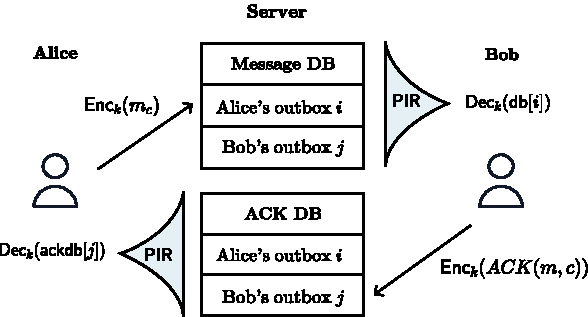
\includegraphics[width=0.7\textwidth]{ACK.pdf}
\caption{All server interactions for a message from Alice to Bob. }
\label{fig:pirandacks}
\end{figure}


Given the limited communication capacity, ACKs turn out to be slightly more subtle than this. In particular, if one user goes offline, we need to continue sending ACKs to them, which could potentially block other ACKs and slow down message transmission. Because each ACK only needs to encode two integers $(m, c)$, we can encode the ACKs for 20 contacts in one database row, which avoids this problem.
\section{Trust establishment}
\label{sec:trustestablishment}

Most existing metadata private messaging systems, such as Pung or Addra, assume that users know beforehand who they wish to talk to, and had a prior key exchange through another channel. In our messaging application, we need a metadata-secure mechanism for the key exchange itself. In other words, if Alice knows the public key $pk_B$ of Bob, then Alice should be able to send an ``invitation" to Bob. Bob must be able to retrieve this invitation from the server, and complete a key exchange with Alice. We call this process ``trust establishment".

This problem is known as Oblivious Message Detection(OMD) in \cite{liutromer2021}. The scheme proposed in \cite{liutromer2021} aims to minimize user download size, but it costs each user $\$ 1$ per million messages scanned, which is prohibitive for our messaging application. We provide two alternate methods of trust establishment with better computational cost and security.

In the following two methods, we assume that Alice and Bob's daemons have generated a Curve25519 key exchange keypair $kx = (kx^P, kx^S)$. Their goal is to inform each other of their $kx^P$ to derive a shared secret $sk$.

\subsection{Face-to-face Invitations}
Our first method assumes that Alice and Bob are able to set up a face-to-face meeting with each other, either in person or over zoom. The trust establishment process is a simple key exchange implemented as follows.

1. Alice encodes the plaintext of her key exchange public key $kx_A^P$ and her allocation index $i_A$ into a human-readable story $s_A$. Bob similarly encodes his story $s_B$.

2. Alice and Bob meet. They share their stories, and type the other's story into their own client. 

3. Alice decodes Bob's story to obtain $kx^P_B$ and $i_B$. She computes the shared secret $sk = DH(kx^P_B, kx^S_A)$, and adds $i_B$ to her set of listening indices.\todo{Better name?} Bob does the same. They can now communicate to each other using our PIR transport layer.

Using this method, all interactions between the users do not pass through any third party. Thus, trust establishment can be completed instantly, cheaply, and securely. Our system do require Alice and Bob to be able to set up a meeting and type each other's story manually. To justify this approach, we believe a privacy-conscious Alice would be willing to set up a face-to-face meeting with Bob before sending him sensitive information.

\subsection{Asynchronous Invitation}

\todo{mention key privacy}

Our second method targets the case when Bob does not know about Alice's invitation beforehand. For example, Alice can be a sensitive client who wishes to privately reach out to Bob's company. 

This method consists of three steps. First, Alice sends an encrypted invitation to the server without indicating its recipient. Second, Bob retrieves this invitation via a full database download. Third, Bob informs Alice of his acceptance via an ACK message.

\textbf{To send an invitation}

1. Upon registration, each user's daemon generates an additional invitation keypair $ki = (ki^P, ki^S)$. Bob's daemon computes a ``public id" $id_B$, which contains his invitation public key $ki_B^P$, key exchange public key $kx_B^P$, and allocation $i_B$ encoded in plaintext. It then displays the id on Bob's GUI. Bob posts $id_B$ on his public profile, such as on twitter or on his company's website.

2. When Alice wishes to send an invitation to Bob, she obtains $id_B$ from Bob's public profile, and decodes it to obtain $(i_B, kx_B^P, ki_B^P)$. She drafts an initial message $m_{AB}$ to accompany her invitation. 

3. Alice's daemon periodically sends the key-value pair $(i_A, c_{AB} = \Enc(kx_B^P, id_A \vert m_{AB}))$ to the server\footnote{It is important to redo this encryption each round, otherwise adversaries will observe the same message repeatedly.}, which stores it in a separate \textbf{AsyncInvitationDatabase}. When Alice has no invitations, her daemon sends $(i_A, \Enc(kx^P, id_A))$ for a random public key $kx^P$.

4. As Alice's daemon sends the invitation, it also compute the shared secret with Bob $sk = DH(kx_B^P, kx^S_A)$. It sends Bob a ``control message" $ctm_{AB}$ via our PIR transport layer, and listens for Bob's ACK.

\textbf{To retrieve an invitation}

1. Bob's daemon periodically downloads the entire \textbf{AsyncInvitationDatabase}. It computes $\Dec(kx^S_B, c)$ over all key-value pairs $(i, c)$. If the decryption fails, Bob's daemon ignores this pair. Now suppose $(i, c) = (i_A, c_{AB})$, and the decryption succeeds. Bob's daemon decodes $i = i_A, id_A, m_{AB}$ from the decrypted data, and displays on Bob's GUI that he received an incoming invitation from $id_A$ with message $m_{AB}$.

2. Bob verifies Alice's identity using $id_A$ and $m_{AB}$, for example by checking Alice's public profile. Bob then chooses to either accept or reject the invitation. If Bob rejects the invitation, no further action is performed. 

\textbf{To accept an invitation}

1. If Bob accepts Alice's invitation, Bob's daemon decodes $id_A$ to obtain $kx_A^P$, and computes the shared secret $sk = DH(kx_A^P, kx_B^S)$. It adds $i_A$ to the set of listening indices.

2. Since Alice is sending the control message $ctm_{AB}$ to Bob using the same shared secret $sk$, Bob's daemon will read $ctm_{AB}$ from the PIR database. It sends an ACK to Alice's control message.

3. When Alice's daemon reads Bob's ACK to $ctm_{AB}$ from the PIR ACK database, it displays on Alice's GUI that Bob has accepted Alice's invitation. Alice and Bob can now communicate to each other using our PIR transport layer.

This method achieves metadata security. We hide the timing of the invitation by making the daemon send to and download \textbf{AsyncInvitationDatabase} on a fixed schedule. We hide the recipient of Alice's request since our encryption scheme is key private(\todo{Cite arvid's section}). 

This method offers convenient trust establishment on par with most existing messaging platforms. Its disadvantage is that downloading the entire database is expensive. We estimate that a key-value pair in the \textbf{AsyncInvitationDatabase} take approximately $200\text{B}$. If we have 1 million users, then the whole database will have a size of approximately $200\text{MB}$. Thus, an individual user might wish to only download the database once or twice each day, which saves bandwidth but delays the detection of invitations. On the other hand, a company user could afford downloading the database every second, which takes $200\text{MB}/s$ download bandwidth but can ensure incoming asynchronous invitations get detected almost instantly.

Finally, we note that this method introduces more attack vectors. For example, an attacker might use social engineering to make Alice believe that a fake $id_B$ belongs to Bob, or simply monitor $A$'s traffic to $B$'s public profile. Therefore, we recommend privacy conscious users to use face-to-face invitations whenever possible.
\newpage
\section{Practical Security} \label{sec:practical-security}

The theoretical guarantees in the previous sections — metadata security without needing to trust the server or the network — all assume that the local computer is wholly trusted. As no fancy encryption scheme prevents a preinstalled backdoor, we cannot eliminate the client-side risk. Nevertheless, we can reduce it. This section outlines the mitigations we undertake: reducing the attack surface by modularizing and supply chain protection, eliminating bugs by being open source, securing code distribution and updates, and protecting against non-privileged local malware.

We cannot achieve perfect security without our user's efforts. \textbf{PLEASE DO NOT USE ANYSPHERE FOR SECURITY-CRITICAL USE CASES ON A COMPUTER YOU DO NOT TRUST}. Our request is especially true while we are in beta, and may have bugs.

% The Anysphere client is only as strong and secure as the most vulnerable part of our software supply chain. Software supply chains are an increasingly complex (and brittle) part of the software ecosystem because of a large and growing number of direct and transitive dependencies written across the world. 
% The Anysphere client is designed to handle extreme private and critical communication securely, so our team has enforced a high bar of security for the core of our system. We focused on providing practical protection by significantly reducing the attack surface of our client, ensuring safe updates, and protecting against non-privileged software. 

% A note on the client's security, in the context of our threat model: Anysphere trusts its client's devices. 
% In particular, we trust that the local device is running a correct implementation of our protocol, and the computer comes without pre-installed backdoors. 
% Our model is the bare minimum of trust we must assume, and we think this is reasonable given the intense focus of Apple and many other companies on device security. 
% (Put another way, no encryption schemes we can come up with can secure our client inside a compromised computer.)
% And with this context, we will present our measures to reduce the risk of a compromised Anysphere client.


\subsection{Reducing the attack surface: modularity and supply chain risk}

As illustrated in \cref{fig:systemdiagram}, our client consists of two parts: a UI frontend and a daemon backend. We sandbox the UI so that it is not allowed to talk to the internet. Instead, all messaging goes through the daemon, which contains all security-critical code. Thus, bugs and malicious code on the front-end cannot compromise security.
\begin{figure*}
    \centering
    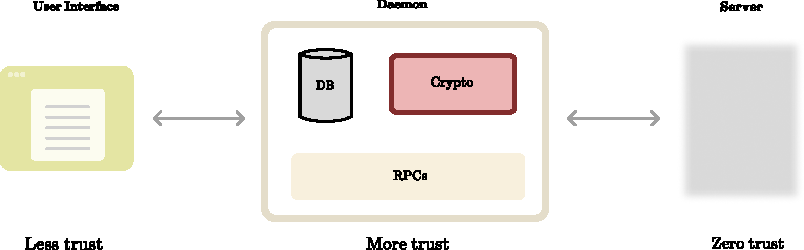
\includegraphics[width=0.9\textwidth]{systemdiagram.pdf}
\caption{System architecture. The UI and the daemon run on your local computer and require some trust assumptions. The UI is cut off from the internet, and can only communicate via the daemon, meaning that it needs lower trust assumptions. The crypto module in the daemon requires the highest level of trust, and uses the widely trusted Libsodium, GRPC, and Sqlite library.}
\label{fig:systemdiagram}
\end{figure*}

We also reduce the attack surface of the daemon. In particular, we ensure a small dependency chain to prevent supply chain attacks. We chose to use \Cpp for all essential daemon code, depending only on a few well-known packages with long-term support and good security practices (Abseil, gRPC, SQLite, Libsodium). We wrote a Rust API for database interactions, being extremely careful with our dependency chain. 

% Many popular languages, including Rust, Go and Python, have great package managers, which led to an ecosystem where packages generally have hundred of transitively dependencies. <- no need to emphasize this?

\subsection{Eliminating bugs: open source}

All code that is required for security is open source. The repositories \\ {\tt \href{https://github.com/anysphere/client}{github.com/anysphere/client}} and  {\tt \href{https://github.com/anysphere/asphr}{github.com/anysphere/asphr}} contain all code for our Daemon and UI. Our server is not open source, since we guarantee security no matter what code is run on our server. 

\subsection{Securing code distribution and updates}

Your computer needs to be running an unmodified copy of our code. For this reason, Anysphere is not a web app —  everytime you visit a website, you give attackers an opportunity to serve you malicious code. Instead, Anysphere is a local app: you can ensure the correct code is downloaded by checking the signature and hash.

%serving code on the web leads to huge vulnerabilities, and should never be done for security-critical codes. The reason is that

%you download the cryptographic code every single time, meaning that every single time you use the website <- [don't think this is true]

Local apps need to be updated. Currently, we use Electron's auto-updater to perform the signature checks for us. We plan to build our own update process, where signatures from two members of our team need to be present for your local app to accept the update. 

%If either of us loses our key, we would not be able to push an update by design. <- [I don't understand this... our team has 3 people.]

\subsection{Protection against non-privileged local malware}

It is unfortunately impossible to prevent compromise from softwares with root privilege. We can, nevertheless, reduce the risk of non-privileged malware. Our beta version does not protect against non-privileged malware, but in the future, we are planning to encrypt the local database, require a password to unlock the app, and use OS-level access controls to make sure only certain processes can access the daemon.

%Again, we do not aim to eliminate the risk here. Once an attacker has access to your computer, it is very, very hard to shield yourself from them.
\section{Related Research}

Cryptography researchers have been studying metadata-private communication for decades. In 1981, David Chaum introduced \textit{mix-nets}, which bounce messages between a small number of servers. Combined with onion encryption, mix-nets make it impossible to determine the destination of a given source packet, \textit{assuming that at least one server is honest}. Using mix-nets, Tor was created in 2002 and became one of the most successful privacy-protecting real-world projects \cite{dingledine2004tor}. Unfortunately, in addition to the server trust issue, mix-nets leak timing data, making it easy for someone with ISP-level network control to observe who is talking to whom. In today's world, it is getting easier and easier to amass enough data to perform such correlation attacks, making mix-net-based approaches unsuitable for absolute security \cite{karunanayake2021anonymisation}.

Systems with stronger metadata-privacy guarantees saw a flurry of interest in the last decade: Dissent and Riposte \cite{corrigan2010dissent,corrigan2015riposte} used so-called DC-nets, Vuvuzela, Atom, Talek and many others \cite{van2015vuvuzela,cheng2020talek,kwon2017atom} introduced mix-nets with stronger security guarantees, Clarion, mcMix and Blinder \cite{alexopoulos2017mcmix,eskandarian2021clarion,abraham2020blinder} introduced multi-party computation techniques, NIAR \cite{shi2021non,bunz2021non} introduced function-hiding functional encryption.
All but NIAR's approach are less secure than our PIR-based approach, and NIAR is impractical at scale due to computation time.
The PIR line of work, started by Angel with Pung \cite{angel2016unobservable,angel2018pir} and continued by Addra \cite{ahmad2021addra}, promises both perfect security and reasonable scalability.

A modern communication system depends on more than just message transmission. There has been much less attention in the literature to other components: establishing trust, handling arbitrary failures, and distributing code securely, to name a few. For trust establishment, Liu and Tromer recently initiated work on oblivious message retrieval (OMR) \cite{liutromer2021}, which is unfortunately not scalable enough for us, but a good start to a field we want to develop further.
\section{What's Next?}

Anysphere has just begun operations, and we are devoted to truly free communication. 
We aim to supervise and help build technologies that allow internet communication without unfair security assumptions.
There are several important milestones that we have set for ourselves to reach to make this genuinely possible; some that are essential in the short-term and others that we want to achieve over a longer time horizon with time and effort.

\subsection{Short term milestones}
\begin{itemize}
  \item \textbf{Group-chats through broadcasting}: An essentially important problem to solve is to allow groups of people to broadcast messages to each other, without depending on the presense of any specific user. We understand that this brings risks in itself to users because it increases the overall risk surface that a user has to trust but we believe it is crucial for large-scale pragmatic adoption.

  \item \textbf{Files and Images}: We hope to allow the sending of small files and images, through our current protocol. Larger files and images are tricky because they expload in the number of chunks needed to deliver them, but we will tackle that problem in due-time.

  \item \textbf{Denial of Service Protection}:

  \item \textbf{Forward Secrecy}

  \item \textbf{Public Key Infrastructure for Anysphere}
\end{itemize}

\subsection{Long-term milestones}
\begin{itemize}
  \item \textbf{Calls}

  \item \textbf{}
\end{itemize}




\printbibliography


\end{document}
